\documentclass[border=16pt]{standalone}
\usepackage{amsmath}
\usepackage{tikz}
\usetikzlibrary{arrows.meta, positioning, calc, backgrounds, fit}

\begin{document}
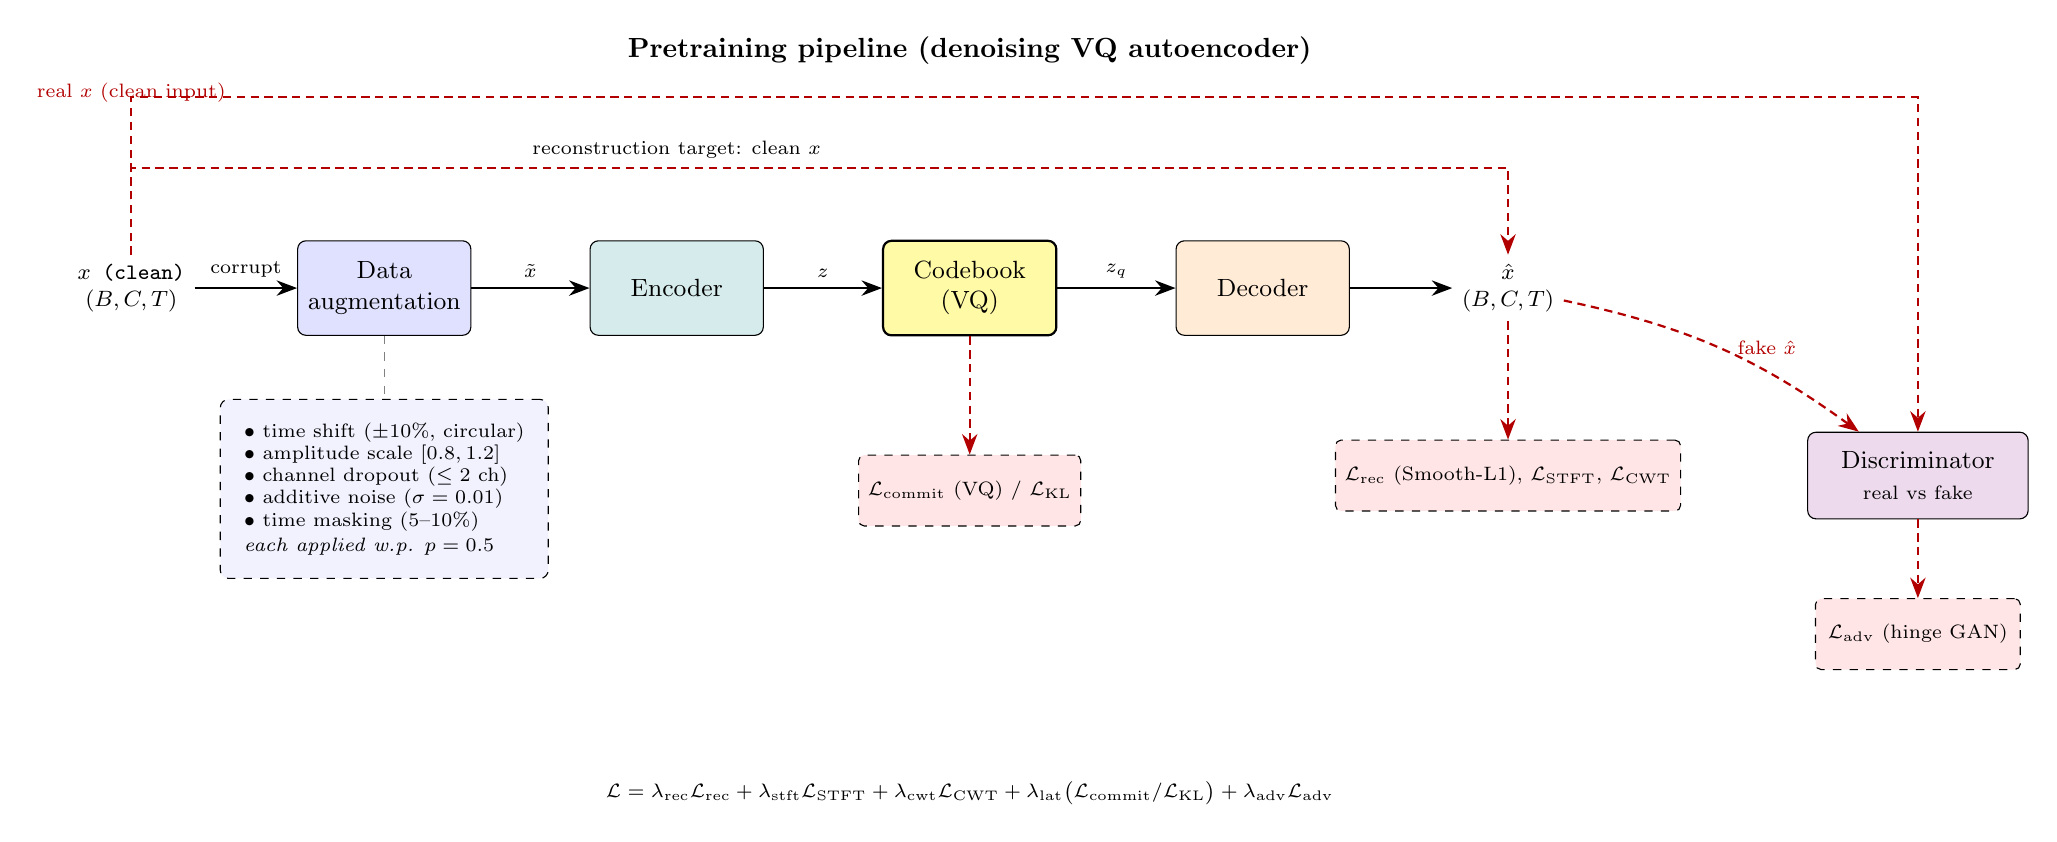
\begin{tikzpicture}[
    font=\small,
    >={Stealth[length=2.6mm]},
    io/.style   = {align=center, font=\ttfamily\footnotesize},
    block/.style= {draw, rounded corners=3pt, align=center, minimum width=22mm,
                   minimum height=12mm},
    enc/.style  = {block, fill=teal!16},
    dec/.style  = {block, fill=orange!16},
    code/.style = {block, fill=yellow!35, thick},
    aug/.style  = {block, fill=blue!12},
    list/.style = {draw, dashed, rounded corners=3pt, align=left, fill=blue!5,
                   font=\scriptsize, inner sep=3mm},
    disc/.style = {draw, rounded corners=3pt, align=center, fill=violet!14,
                   minimum width=28mm, minimum height=11mm},
    loss/.style = {draw, dashed, rounded corners=2pt, align=center, fill=red!10,
                   minimum height=9mm, minimum width=26mm, font=\scriptsize},
    flow/.style = {->, thick},
    lossflow/.style = {->, thick, densely dashed, red!70!black},
]

% ================= main forward pipeline =================
\node[io]   (xc)  {$x$ (clean)\\$(B,C,T)$};
\node[aug]  (aug) [right=13mm of xc]  {Data\\augmentation};
\node[enc]  (enc) [right=15mm of aug] {Encoder};
\node[code] (cb)  [right=15mm of enc] {Codebook\\(VQ)};
\node[dec]  (dec) [right=15mm of cb]  {Decoder};
\node[io]   (xh)  [right=13mm of dec] {$\hat{x}$\\$(B,C,T)$};

\draw[flow] (xc)  -- node[above,font=\scriptsize]{corrupt} (aug);
\draw[flow] (aug) -- node[above,font=\ttfamily\scriptsize]{$\tilde{x}$} (enc);
\draw[flow] (enc) -- node[above,font=\ttfamily\scriptsize]{$z$} (cb);
\draw[flow] (cb)  -- node[above,font=\ttfamily\scriptsize]{$z_q$} (dec);
\draw[flow] (dec) -- (xh);

% ================= title =================
\node[font=\bfseries] at ($(cb.north)+(0,24mm)$)
    {Pretraining pipeline (denoising VQ autoencoder)};

% ================= reconstruction target (denoising) =================
\coordinate (top) at ($(xc.north)+(0,11mm)$);
\draw[lossflow] (xc.north) |- (top) -| (xh.north);
\node[font=\scriptsize, above] at (top -| enc) {reconstruction target: clean $x$};

% ================= corruptions list =================
\node[list] (auglist) [below=8mm of aug]
    {$\bullet$ time shift ($\pm10\%$, circular)\\
     $\bullet$ amplitude scale $[0.8,1.2]$\\
     $\bullet$ channel dropout ($\leq 2$ ch)\\
     $\bullet$ additive noise ($\sigma=0.01$)\\
     $\bullet$ time masking ($5\text{--}10\%$)\\[1pt]
     {\itshape each applied w.p. $p=0.5$}};
\draw[dashed, gray] (aug.south) -- (auglist.north);

% ================= losses =================
\node[loss] (lcom) [below=15mm of cb]
    {$\mathcal{L}_{\text{commit}}$ (VQ)\ /\ $\mathcal{L}_{\text{KL}}$};
\draw[lossflow] (cb) -- (lcom);

\node[loss] (lrec) [below=15mm of xh]
    {$\mathcal{L}_{\text{rec}}$ (Smooth-L1),\ $\mathcal{L}_{\text{STFT}}$,\ $\mathcal{L}_{\text{CWT}}$};
\draw[lossflow] (xh) -- (lrec);

% adversarial branch: D receives the clean input (real) and the reconstruction (fake)
\node[disc] (disc) [right=16mm of lrec] {Discriminator\\{\scriptsize real vs fake}};
\node[loss] (ladv) [below=10mm of disc] {$\mathcal{L}_{\text{adv}}$ (hinge GAN)};

\draw[lossflow] (xh) to[bend left=12]
    node[right=1mm, font=\scriptsize]{fake $\hat{x}$} (disc);
\draw[lossflow] (xc.north) -- ++(0,20mm)
    node[above, pos=0.9, font=\scriptsize]{real $x$ (clean input)} -| (disc.north);
\draw[lossflow] (disc) -- (ladv);

% ================= total loss =================
\node[align=center, font=\scriptsize] at ($(cb.south)+(0,-58mm)$)
    {$\mathcal{L}=\lambda_{\text{rec}}\mathcal{L}_{\text{rec}}
      +\lambda_{\text{stft}}\mathcal{L}_{\text{STFT}}
      +\lambda_{\text{cwt}}\mathcal{L}_{\text{CWT}}
      +\lambda_{\text{lat}}\big(\mathcal{L}_{\text{commit}}/\mathcal{L}_{\text{KL}}\big)
      +\lambda_{\text{adv}}\mathcal{L}_{\text{adv}}$};

\end{tikzpicture}
\end{document}
